\documentclass[]{beamer}
\usepackage[T1]{fontenc}
\usepackage[utf8]{inputenc}
\usepackage{lmodern}
\usepackage[italian]{babel}
\usepackage{mathrsfs}
\usepackage{cancel}

\title{Meccanica dei fluidi}
\author{\texorpdfstring{Mattia Cozzi\newline\href{mailto:cozzimattia@gmail.com}{\texttt{cozzimattia@gmail.com}}}{Mattia Cozzi}}
\date{a.s.~2023/2024}

%\documentclass[handout]{beamer}     %usare questa classe per generare l'handout
%\usepackage{pgfpages}   %per mostrare più quadri nella stessa pagina
%\pgfpagesuselayout{4 on 1}[a4paper,border shrink=5mm,landscape]
\usetheme{Singapore}
%\useoutertheme[left]{sidebar} %elementi intorno alle diapositive
\setbeamercovered{dynamic} %modifica l'aspetto del testo grigetto delle diapositive future. Argomenti: invisible/transparent/dynamic
\usecolortheme{orchid}
%COLORE PRINCIPALE
\definecolor{marroncino}{RGB}{156, 26, 0} % UBC Blue (primary)
\setbeamercolor{structure}{fg=marroncino} % itemize, enumerate, etc

\theoremstyle{plain}
\newtheorem{teorema}{Teorema}

\usepackage{tikz}
\usepackage{circuitikz}

\usepackage{pgf,pgfplots,graphicx}
\usetikzlibrary{angles,quotes,arrows,shapes,decorations.markings}
\pgfplotsset{compat=1.15}
\usepgfplotslibrary{units,fillbetween} % to add units easily to axis

\newcommand{\fem}{f_{em}}

\def\angolo[#1](#2)(#3:#4:#5)% Syntax: [draw options] (center) (initial angle:final angle:radius)
    { \draw[#1] ($(#2)+({#5*cos(#3)},{#5*sin(#3)})$) arc (#3:#4:#5); }


\newcommand<>{\xxcancel}[1]{\alt#2{\xcancel{#1}\vphantom{#1}}{#1}}

\begin{document}

\begin{frame}
  \titlepage
\end{frame}





\begin{frame}
\frametitle{Contenuti}
\tableofcontents
\end{frame}


\section{Fluidi}

\begin{frame}
\frametitle{Stati della materia}
La materia (composta da atomi, che formano molecole), può presentarsi in tre stati:
\begin{figure}
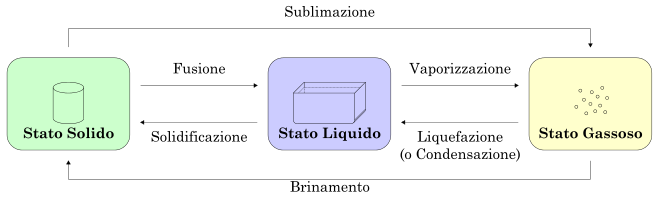
\includegraphics[width=.9\columnwidth]{img/passaggidistato.png}
\end{figure}
\begin{columns}
\begin{column}{0.3\textwidth}
\begin{center}
I solidi hanno volume e forma propria.\\~
\end{center}
\end{column}
\begin{column}{0.3\textwidth}
\begin{center}
I liquidi hanno un volume, ma non una forma propria.\\~
\end{center}
\end{column}
\begin{column}{0.3\textwidth}
\begin{center}
I gas occupano tutto lo spazio del recipiente che li contiene.
\end{center}
\end{column}
\end{columns}
\end{frame}



\begin{frame}
\frametitle{Fluidi}
Un \alert<1>{fluido} è un sistema facilmente deformabile, che non ha una forma propria ma assume quella del recipiente che lo contiene.\pause

~

Liquidi e gas sono dei fluidi, e si distinguono per l'intensità delle \alert<2>{forze di coesione} tra le particelle costituenti.\pause

~

Nei liquidi, le particelle sono molto più vicine tra loro, e pertanto i liquidi hanno densità molto maggiori dei gas.
\end{frame}

\section{Pressione}

\begin{frame}
\frametitle{La pressione}
Immaginiamo di ``spingere'' dell'acqua o dell'aria e ci rendiamo conto che nel caso dei fluidi il concetto dinamico di \emph<1>{forza} non è più sufficiente.\pause

~

Per ottenere lo stesso risultato dinamico di una forza in un fluido è necessario che la forza venga distribuita su tutti i punti della superficie del fluido.\pause

~

Introduciamo la \alert<3>{pressione}:
\begin{center}
\colorbox{marroncino!30}{$ p = \dfrac{F}{S} $} ~~~~~~ $ [ Pa ] = \left[ \dfrac{N}{m^2} \right] $
\end{center}
dove $ F $ è la forza che preme perpendicolarmente alla superficie del fluido.
\end{frame}


\begin{frame}
\frametitle{Esercizio}
\begin{exampleblock}{Calcolo della pressione}
  Un cubo di alluminio ($ d = 2,70 \times 10^{3} \, kg/m^3 $) di lato $ \ell = 2,5 \, cm $ è appoggiato a terra.

  Calcola la pressione esercitata dal cubo sul pavimento.
\end{exampleblock}\pause

~

La forza esercitata è la forza peso, per la quale abbiamo bisogno della massa, che otteniamo a partire dalla densità e dal volume:
\begin{center}
  $ d = \dfrac{m}{V} \qquad \Longrightarrow \qquad m = dV  $
\end{center}\pause
La pressione sarà:
\begin{center}
  $ p = \dfrac{F}{S} = \dfrac{P}{S} = \dfrac{mg}{\ell^2} = \dfrac{dVg}{\ell^2} = \dfrac{d\ell^3g}{\ell^2} = d\ell g $
\end{center} 

\end{frame}


\begin{frame}
\frametitle{Il principio di Pascal}
Blaise Pascal (1623-1662) dimostrò che:
\begin{block}{Principio di Pascal}
Quando si esercita una pressione su un fluido chiuso in un recipiente,
essa si trasmette inalterata in ogni punto del fluido. In particolare, la pressione è sempre perpendicolare alle pareti del recipiente.
\end{block}
\begin{figure}
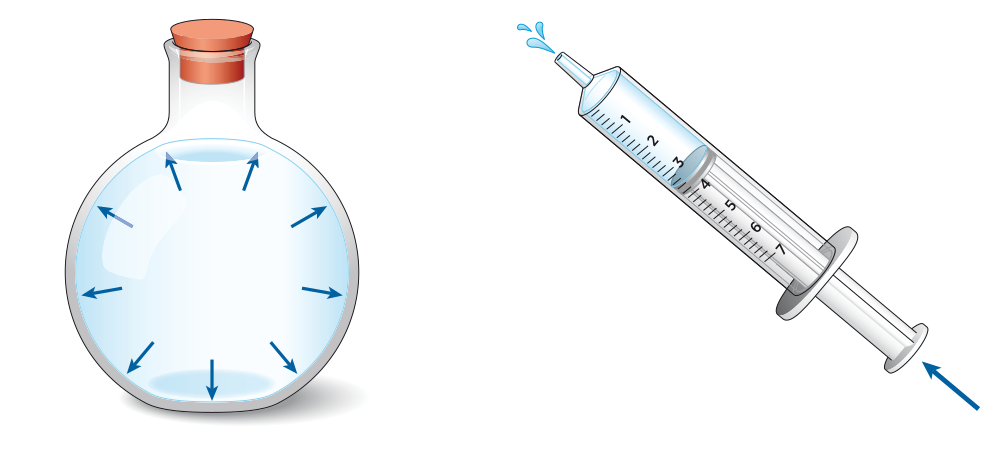
\includegraphics[width=.5\columnwidth]{img/principiopascal.png}

\href{video/Pascal.mp4}{\beamergotobutton{Video: Principio di Pascal}}
\end{figure}
\end{frame}

\begin{frame}
\frametitle{Applicazioni del principio di Pascal}
Se due parti di un fluido sono a contatto con superfici mobili (pistoni) con area $ A_1 \gg A_2 $, allora:
\begin{center}
$ p_1 = p_2 $~~~\pause$ \Longrightarrow  $~~~$ \dfrac{F_1}{A_1} = \dfrac{F_2}{A_2} $\pause~~~$ \Longrightarrow  $~~~\colorbox{marroncino!30}{$ F_1 = \dfrac{A_1}{A_2}F_2 $}
\end{center}
\alert<3>{La forza sul pistone più grande è molto più intensa della forza sul pistone più piccolo}.
\begin{columns}
\begin{column}{0.3\textwidth}
\visible<4->{\begin{figure}
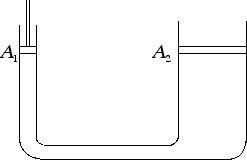
\includegraphics[width=\columnwidth]{img/sollevatore.jpg}
\end{figure}}
\end{column}
\begin{column}{0.3\textwidth}
\visible<5->{\begin{figure}
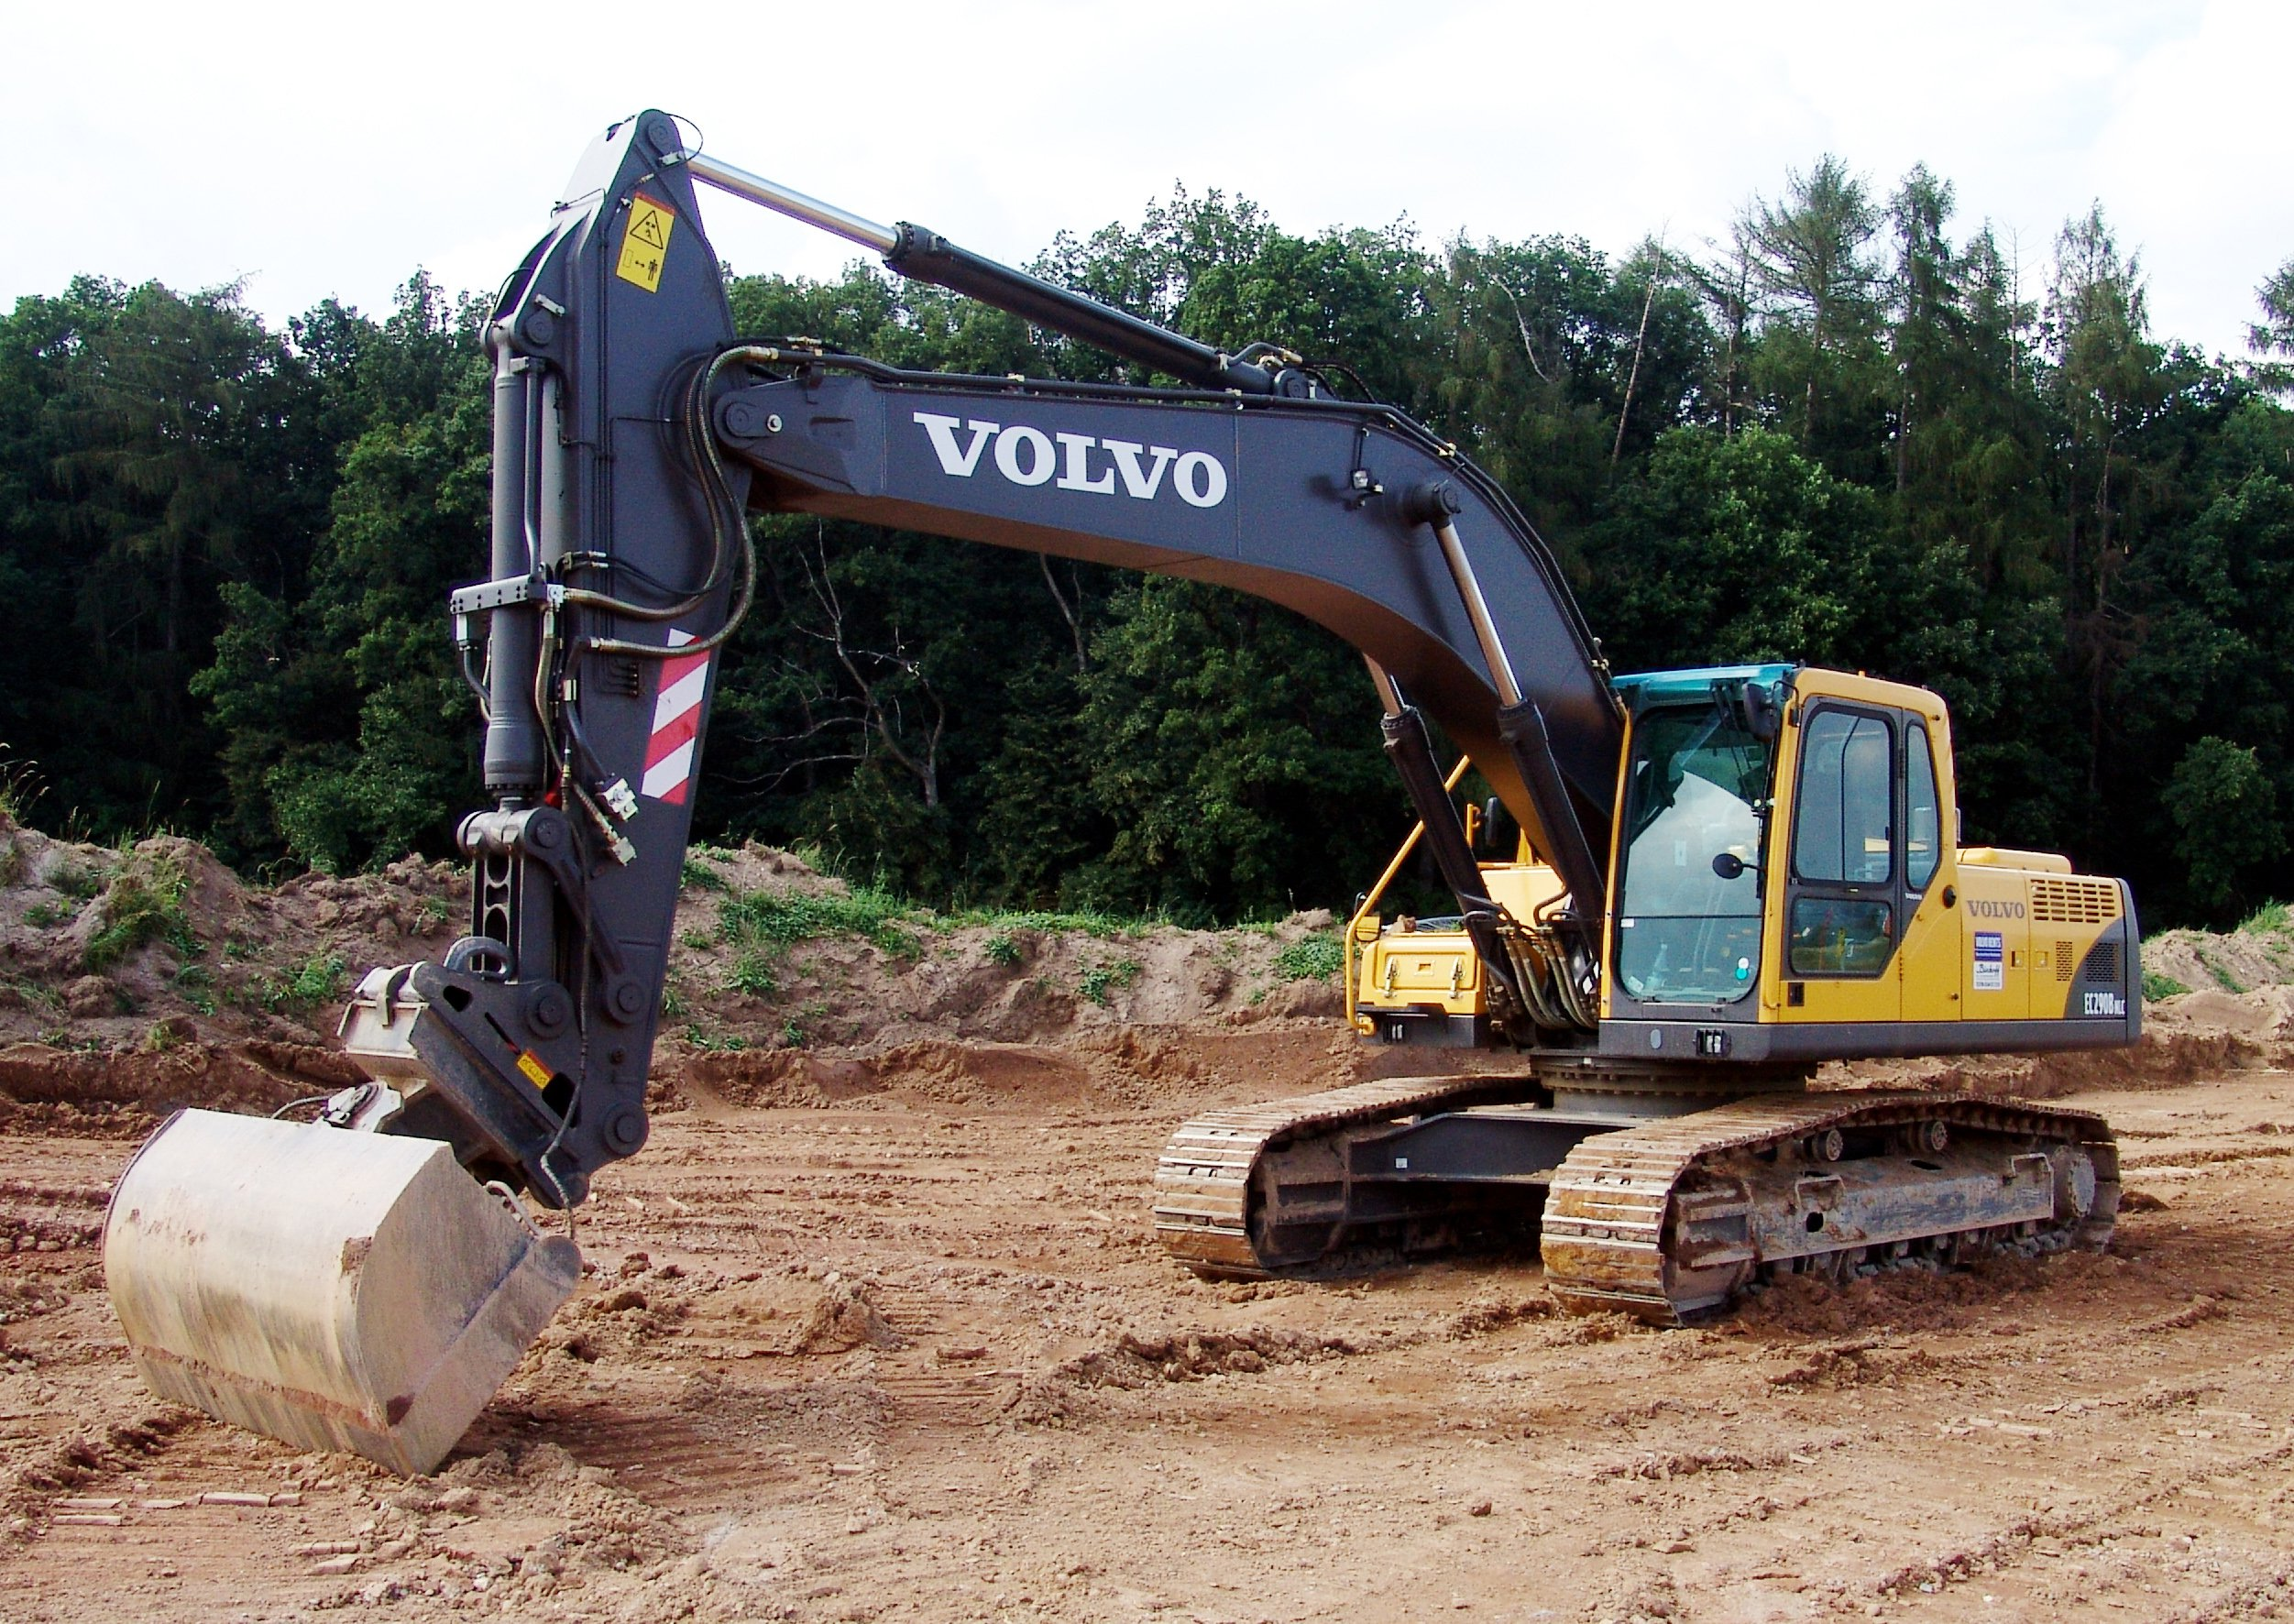
\includegraphics[width=\columnwidth]{img/escavatore.jpg}
\end{figure}}
\end{column}
\begin{column}{0.3\textwidth}
\visible<6->{\begin{figure}
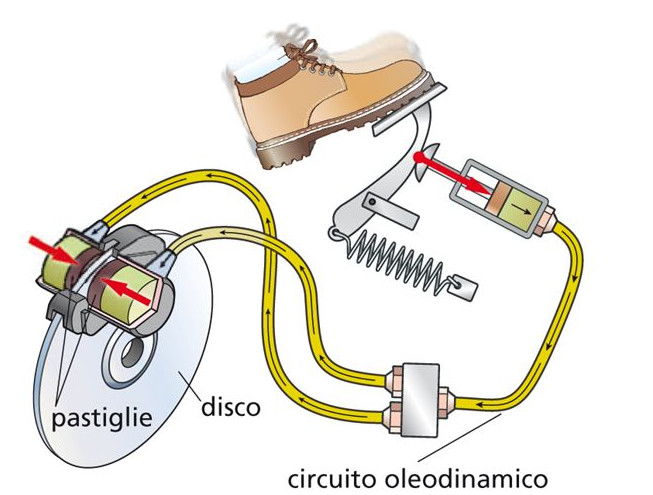
\includegraphics[width=\columnwidth]{img/freni.jpg}
\end{figure}}
\end{column}
\end{columns}
\end{frame}



\begin{frame}
\frametitle{Esercizio}
\begin{exampleblock}{Calcolo della forza}
  Una forza di $ 150 \, N $ è applicata su un pistone circolare di raggio $ r_1 = 3,00 \, cm $, collegato idraulicamente ad un altro pistone più grande, di raggio $ r_2 = 5,00 \, cm $.

  Calcola la forza che il pistone maggiore riesce ad esercitare.\hspace*{\fill}[$ 417 \, N $]
\end{exampleblock}
\end{frame}





\begin{frame}
\frametitle{La pressione atmosferica}

\begin{columns}
\begin{column}{0.4\textwidth}
\begin{center}
\begin{figure}
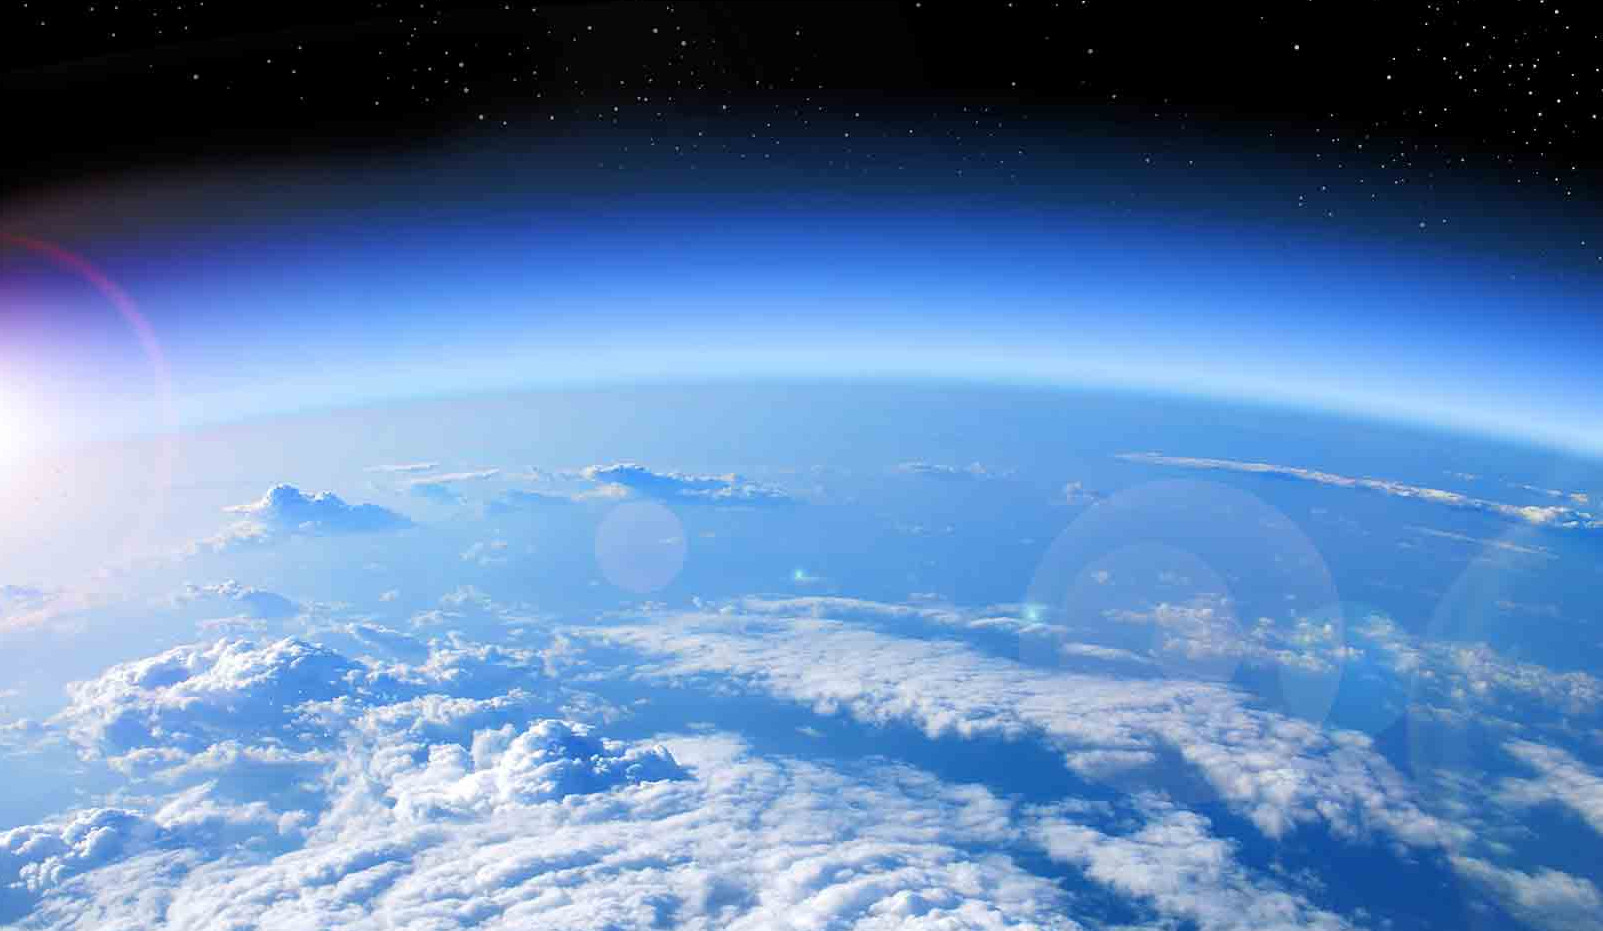
\includegraphics[width=\columnwidth]{img/atmosfera.jpg}
\end{figure}
\end{center}
\end{column}
\begin{column}{0.45\textwidth}
L’atmosfera è l’involucro gassoso che circonda la Terra, trattenuto dalla forza di gravità.
\end{column}
\end{columns}\pause

~

~

L'atmosfera esercita una forza su tutti i corpi che vi sono immersi, la \alert{pressione atmosferica} (misurata con precisione per la prima volta da Evangelista Torricelli nel 1643).
\begin{center}
\colorbox{marroncino!30}{$ p_0 = 1 \, atm = 101\, 325 \, Pa \sim 1,01 \times 10^5 \, Pa $}
\end{center}
\end{frame}

\begin{frame}
\frametitle{La pressione idrostatica}
Un liquido in quiete ha un peso, e tale peso è una forza che esercita una pressione in ogni punto del liquido.\pause

~

Tale pressione dipende dalla profondità a cui ci si trova e dalla densità del fluido:
\begin{center}
\colorbox{marroncino!30}{$ p = \rho g h $} ~~~~~~ Legge di Stevino
\end{center}\pause
Se consideriamo anche la pressione atmosferica che preme sul liquido:
\begin{center}
\colorbox{marroncino!30}{$ p = \rho g h + p_0 $}
\end{center}
\end{frame}


\begin{frame}
\frametitle{Vasi comunicanti}
Una conseguenza della legge di Stevino è che un liquido, contenuto in due o più contenitori comunicanti tra loro, in presenza di gravità, raggiunge la stessa altezza in ogni contenitore.

\begin{figure}
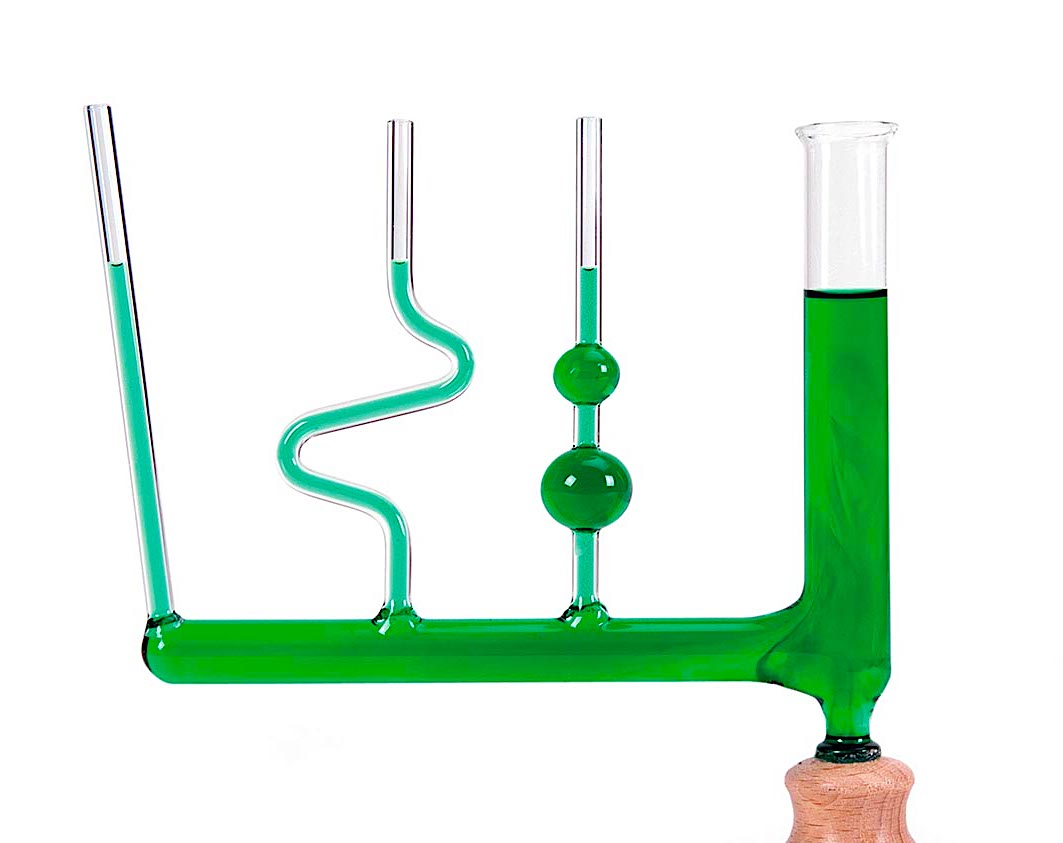
\includegraphics[width=.5\columnwidth]{img/vasicomunicanti.jpg}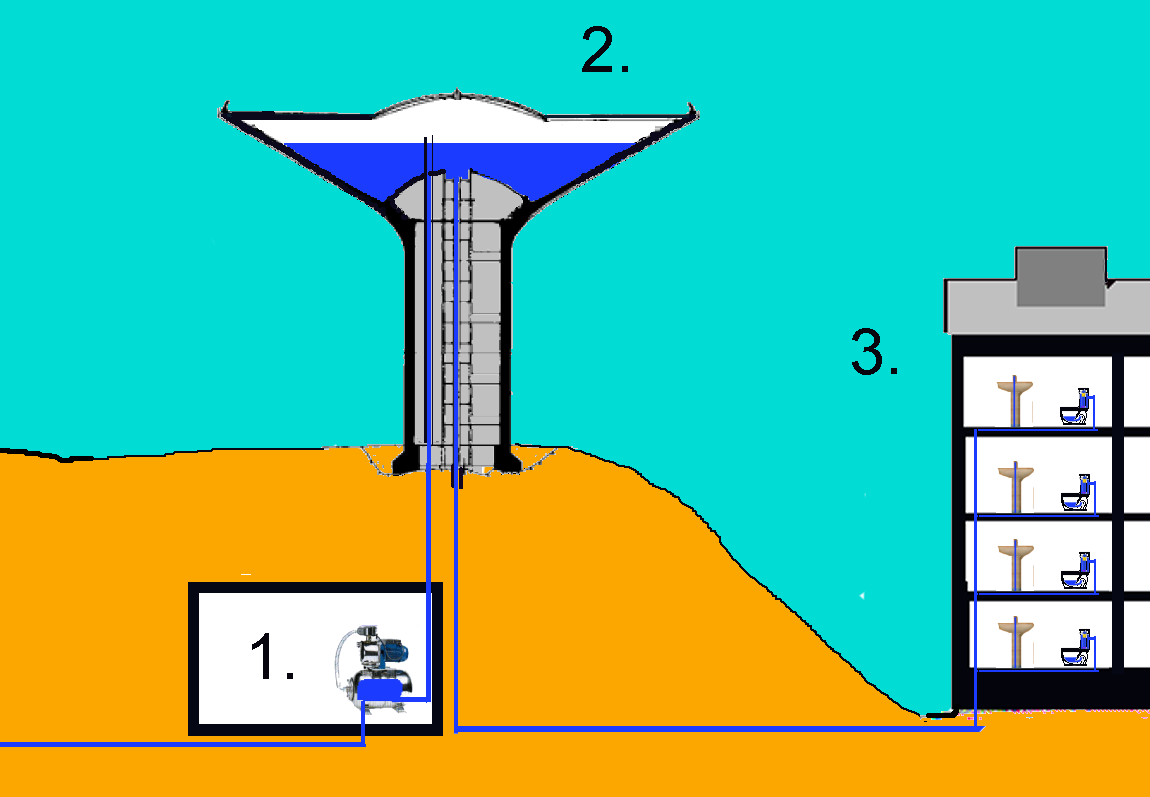
\includegraphics[width=.5\columnwidth]{img/acquedotto.png}
\end{figure}
\end{frame}

\begin{frame}
\frametitle{Esercizio}
\begin{exampleblock}{Calcolo della pressione}
  Calcola la pressione totale esercitata su un paio di occhialini di dimensioni $ 30 \, cm^2 $ posti sul fondo di una piscina profonda $ 300 \, cm $. La densità dell'acqua è $ 1,00 \times 10^{3} \, kg/m^3 $.\hspace*{\fill}[$ 1,3 \times 10^5 \, Pa $]
\end{exampleblock}
\end{frame}

\section{Archimede}


\begin{frame}
\frametitle{La spinta idrostatica}
Il galleggiamento dei corpi è dovuto alla spinta che essi ricevono da parte dell'acqua.

\begin{block}{Principio di Archimede}
Un corpo immerso (totalmente o parzialmente) in un fluido riceve una spinta  verso l'alto di intensità pari al peso di una massa di fluido di volume uguale a quella della parte immersa del corpo.

~

Più semplicemente, possiamo affermare che \alert{un corpo immerso in un fluido riceve una spinta dal basso verso l'alto pari al peso del volume di fluido spostato}.
\end{block}
\end{frame}



\begin{frame}
\frametitle{Pressione a diverse profondità e forza totale sul corpo}
\begin{figure}
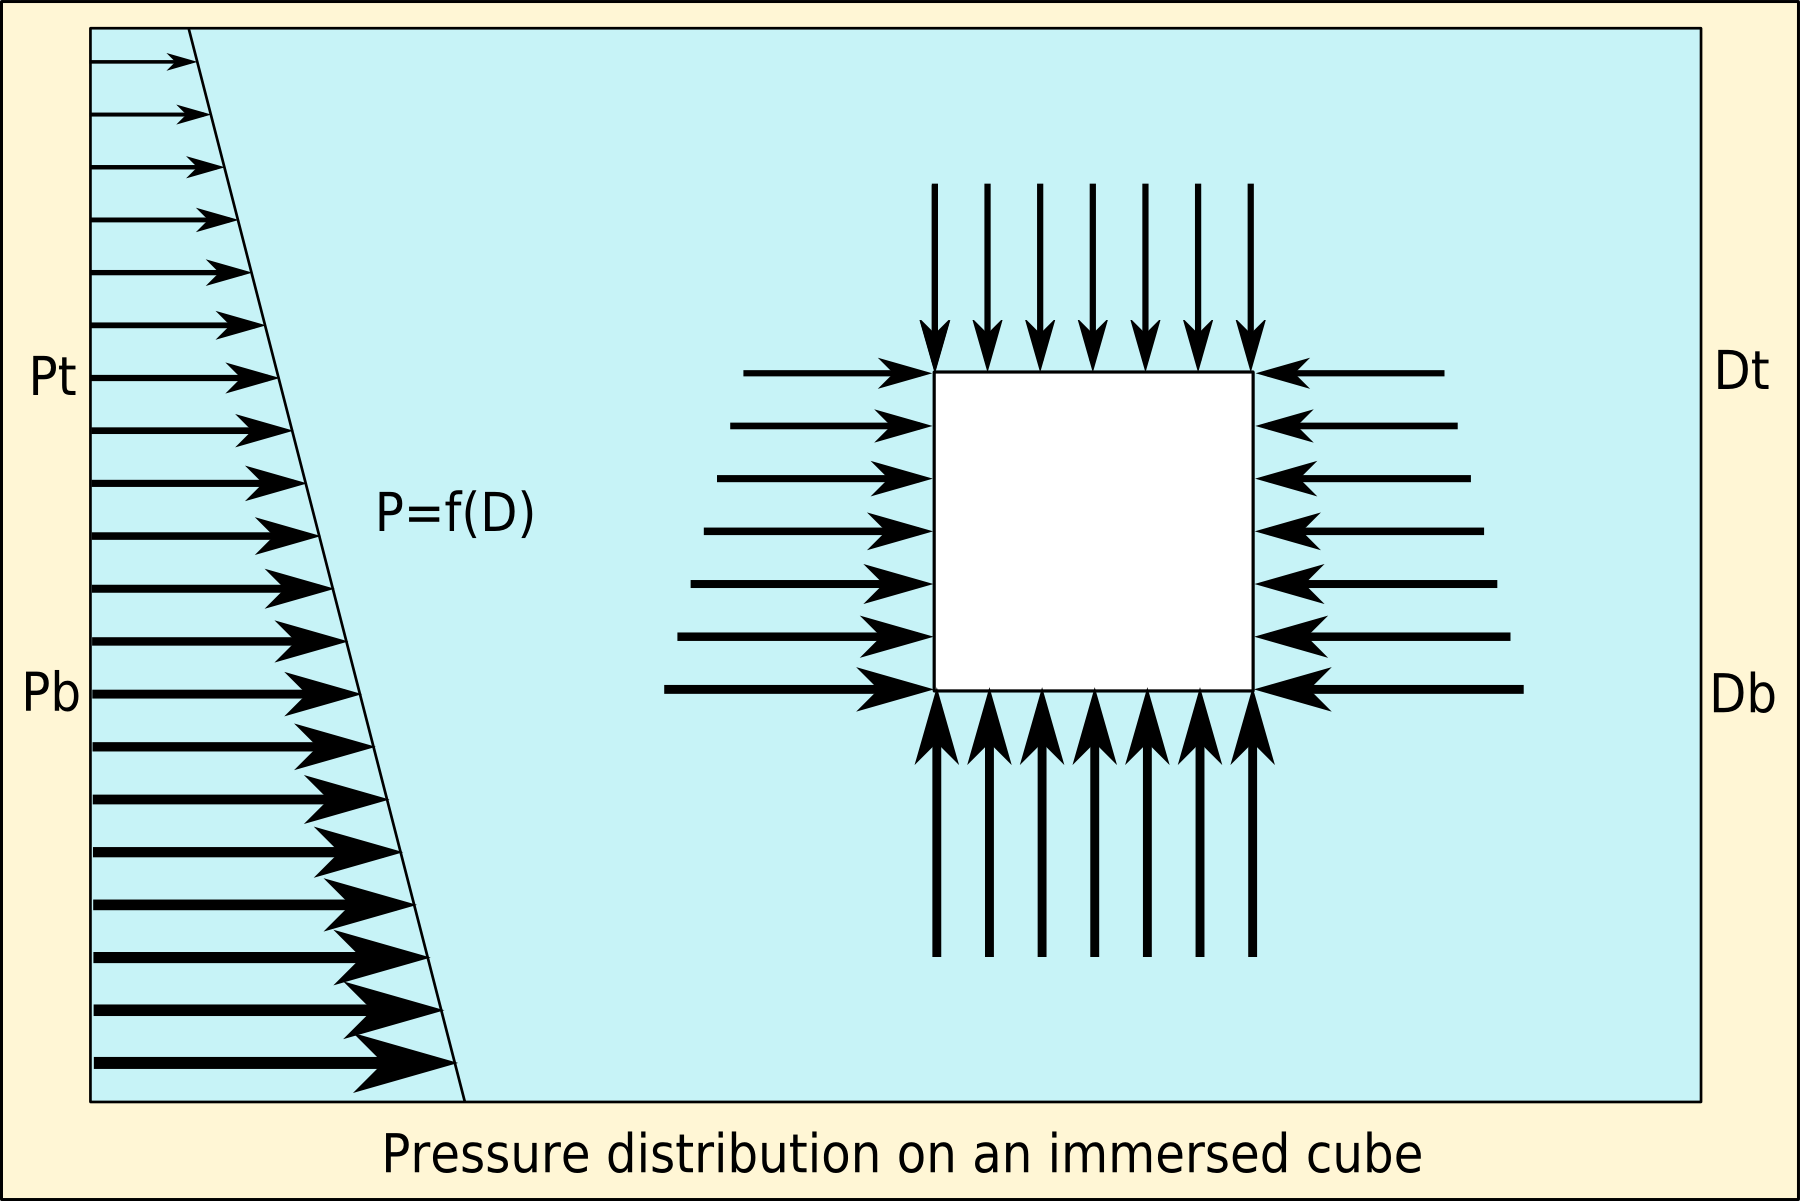
\includegraphics[width=.7\columnwidth]{img/archimede.png}
\end{figure}
Possiamo intuire che anche la spinta di Archimede è una conseguenza della legge di Stevino.
\end{frame}


\begin{frame}
\frametitle{Calcolo della spinta di Archimede}
Secondo il principio di Archimede, se indichiamo con $ S $ la spinta verso l'alto:
\begin{center}
$ S = P_{fluido} = m_{fluido}  g $
\end{center}\pause
Poiché $ m_{fluido} = \rho_{fluido}  V_{fluido} $ allora:
\begin{center}
$ S = \rho_{fluido}  V_{fluido}  g $
\end{center}\pause
Tuttavia, $ V_{fluido} = V_{immerso} $, e pertanto:
\begin{center}
\colorbox{marroncino!30}{$ S = \rho_{fluido}  V_{immerso}  g $}
\end{center}
\end{frame}


\begin{frame}
\frametitle{Condizione di galleggiamento}
Un corpo galleggia se la spinta idrostatica è maggiore o uguale alla sua forza peso.
\begin{center}
$ S \geq P $
\end{center}\pause
\begin{center}
$ \rho_{f}  V_{c}  \cancel{g} \geq m_{c} \cancel{g} $
\end{center}\pause
\begin{center}
$ \rho_{f} \cancel{V_{c}} \geq \rho_{c} \cancel{V_{c}} $
\end{center}\pause
\begin{center}
\colorbox{marroncino!30}{$ \rho_{f}  \geq \rho_{c}  $}
\end{center}\pause
Se $ \rho_{f} < \rho_{c}  $, il corpo affonda (ma avrà un \emph{peso relativo} minore).
\end{frame}




\begin{frame}
\frametitle{Esercizio}
\begin{exampleblock}{Calcolo del peso relativo}
  Un masso con un volume $ V = 1,20 \, m^3 $ e densità $ d = 4,550 \times 10^{3} \, kg/m^3 $ si trova sul fondo di un lago contenente acqua dolce.
  
  Calcola il suo peso relativo. \hspace*{\fill}[$ 4,18 \times 10^5 \, N $]
\end{exampleblock}
\end{frame}


\begin{frame}
\frametitle{Corpi parzialmente immersi}
Se la spinta è maggiore del peso, il corpo galleggia.

~

Quando un corpo galleggia si ha una condizione di equilibrio tra il peso del corpo e la spinta di Archimede, che dipende unicamente dal volume immerso $ V_i $.

~
\begin{figure}
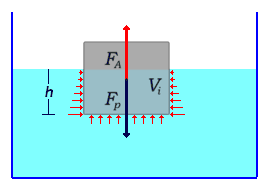
\includegraphics[width=.4\columnwidth]{img/volumeimmerso.png}
\end{figure}
\end{frame}


\begin{frame}
\frametitle{Immersione ed emersione di un sommergibile}
\begin{figure}
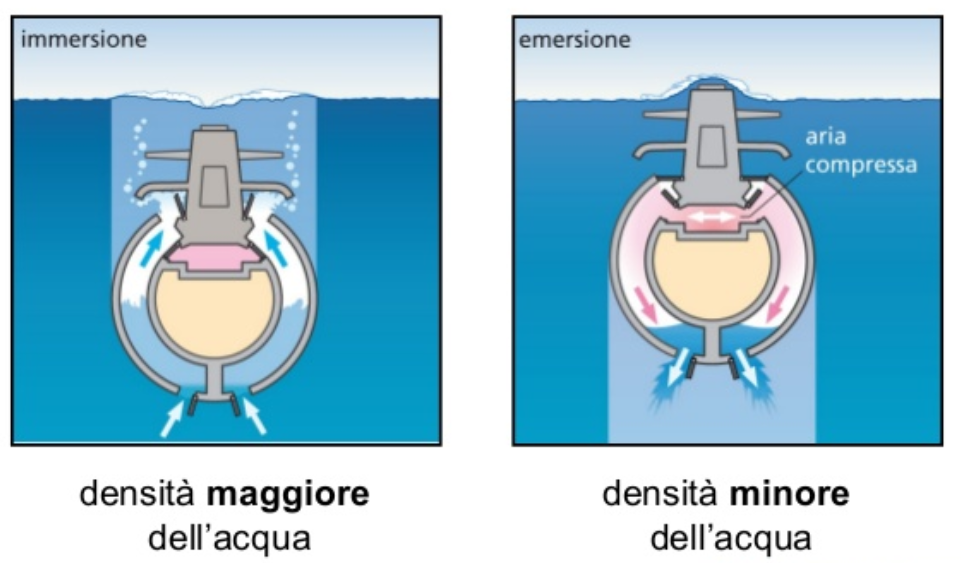
\includegraphics[width=.8\columnwidth]{img/sottomarino.png}
\end{figure}
\end{frame}



\end{document}
